\chapter{ARTE COMPUTACIONAL E INTERATIVIDADE}

Neste capítulo serão apresentados três temas centrais que, no trabalho proposto, aparecem relacionados entre si. São eles: a interatividade, a arte computacional e o universo das instalações interativas. No que tange à interatividade relatamos os caminhos que, do ponto de vista do espectador, foram percorridos na arte até, finalmente, chegarmos na interação. Além disso, exploramos os diferentes graus de interatividade propostos por autores desde \citeauthoronline{levy}, que propõe a interatividade no contexto das tecnologias analógicas e digitais, até  \citeauthoronline{primo}, que realiza um estudo da interatividade em ambientes informáticos. Depois, vamos buscar entender o significado da arte computacional e alguns dos fatores que a caracterizam. E, por fim, exploraremos o universo das instalacões interativas e como se dá a relação entre elas e o corpo do observador.




\section{DA CONTEMPLAÇÃO À INTERAÇÃO}

De acordo com \citeonline[p. 97]{frechiani}, historicamente, dentre as tendências que situam a importância do espectador na costituição da obra, a arte percorreu um caminho até finalmente desembocar no universo da interatividade. Esse percurso parte da contemplação, onde o fruidor é um agente passivo, passa pela participação ativa, onde encontramos a manipulação de objetos, até finalmente chegar na interação, onde se manifesta uma relação de reciprocidade entre o usuário e um sistema computacional. Neste processo \citeonline[p. 2570]{vares} afirma que é possível perceber mudanças circunstanciais e definitivas na criação, na produção e, também, na recepção e percepção da obra por parte do espectador. 

Segundo \citeonline[p. 10]{plaza}, foi a partir dos anos cinqüenta que se constituiram, no campo da arte, tendências que traduzem e antecipam as mudanças produzidas pelas tecnologias. Experiências de representações visuais levaram os artistas desta época a interagir com a ciência e a tecnologia sob o nome de arte cinética, utilizando-se da luz, do movimento e da cor, numa tentativa de sistematizar a arte visual, argumenta \citeonline[p. 76]{rahde}. Retomando \citeonline[p. 11]{plaza}, o artista se interessa por uma nova forma de comunicação, onde procura a participação do espectador para elaborar a obra de arte. A obra deixa de ser fruto apenas do artista e se produz no decorrer do diálogo. O espectador não está mais reduzido ao olhar, ele tem a possibilidade de agir sobre a obra e modificá-la. Ainda de acordo com \citeonline[p. 14]{plaza} "a noção de arte de participação tem por objetivo encurtar a distância entre criador e espectador. Na participação ativa o espectador se vê induzido à manipulação e exploração do objeto artístico ou de seu espaço". Vivenciamos o início do deslocamento das atribuições do artista para o fruidor. 

\citeonline[p. 77]{rahde} afirma que nos anos setenta a intervenção do público na obra se tornou um fator natural, já que esta era uma das muitas intenções das obras criadas neste período. Propostas como as da escultora Lygia Clark tornaram possível a desestetização da arte, não importando se os trabalhos se configuravam como obras de arte, mas procurando envolver o espectador nos aspéctos psicológicos da leitura imagística, diz a autora. Acrescenta que na década de oitenta houve uma ruptura em relação às décadas anteriores quando se passou a pesquisar as novas tecnologias, como o computador e o audiovisual, estabelecendo-se verdadeira revolução nas artes. Para \citeonline[p. 53]{caetano2009} inaugura-se a era das interfaces, na qual novos paradigmas são evidenciados a partir da interação homem-máquina. Segundo ela, junto com a proliferação dos computadores pessoais, ocorre a desmistificação das tecnologias computacionais, o que colocou os artistas diante de possibilidades estéticas interativas. "A teoria e o fazer artístico, antes distanciados do apoio da solução científica, encontraram novas formulações, atendo-se mais ao processo do que ao produto final no conceito de obra" \cite[p. 78]{rahde}.

\citeonline{tavares} explica que o fenômeno da interação mediado pelas tecnologias eletrônicas pressupõe a existência de um processo de realimentação, em que cada ação do receptor condiciona uma conseqüente reação da máquina e vice-versa, possibilitando um contínuo diálogo entre esses elementos. A visão computacional tem um grande papel nessa dinâmica pois são os algoritmos que tornam os trabalhos artísticos mais dinâmicos, imersivos e fazem com que o espectador se constitua como parte do trabalho. Como visão computacional compreende-se a definição proposta por \citeonline[p. 134]{caetano} que diz que "é a forma pela qual 'o computador enxerga' e 'interpreta as imagens', um conjunto de dados numéricos digitais, uma matriz numérica digital descrevendo qualquer conjunto imagético fisicamente contextualizado".

\citeonline[p. 2566]{rabello2011} relata que os artistas tem proporcionado novos mundos ao estabelecer diálogos e projetar novas realidades, propondo obras que ultrapassam o modelo de objeto pronto para um modelo dinâmico e em constante transformação, o que possibilita ao público um território de experiência ampliado por meio da simbiose entre homem e máquina.

Para \citeonline[p. 22]{domingues} a arte interativa é, portanto, completamente avessa ao principio da inércia. Surge um novo espectador que, através das interfaces, tem acesso a obra proposta. Ainda de acordo com a autora, são as interfaces amigáveis que permitem as trocas do espectador com as fontes de informação. A contemplação é substituída pela relação. Assim, \citeonline[p. 20]{plaza} conclui que uma obra de arte interativa é um espaço latente e suscetível a todos os prolongamentos sonoros, visuais e textuais. O cenário programado pode se modificar em tempo real ou em função da resposta dos operadores. A interatividade não é somente uma comodidade técnica e funcional; ela implica física, psicológica e sensivelmente o espectador em uma prática de transformação. O destinatário potencial torna-se co-autor e as obras tornam-se um campo aberto a múltiplas possibilidades e suscetível a desenvolvimentos imprevistos numa co-produção de sentidos.


\subsection{GRAUS DE INTERATIVIDADE}

A partir de estudos dos trabalhos de autores como \citeonline{levy, couchot, tavares, bochio, primo, souza} podemos classificar a interatividade de diferentes maneiras. Tomemos como ponto de partida o trabalho de \citeonline[p. 81]{levy} onde afirma que o termo interatividade, em geral, ressalta a participação ativa do beneficiário de uma transação de informação. Acrescenta que um receptor da informação nunca é completamente passivo: ele decodifica, interpreta, mobiliza seu sistema nervoso de muitas maneiras, e sempre de forma diferente de outra pessoa. Trazendo com isso o que chama de grau de interatividade, que, segundo ele, é distinto para cada mídia ou dispositivo de comunicação e pode ser medido em eixos diferentes, são eles  \cite[p. 82]{levy}:

\begin{enumerate}
  \item As possibilidades de apropriação e de personalização da mensagem recebida, que podem ser linear, em rede, em fluxo, em mundo virtual;
  \item A reciprocidade da comunicação, que pode ser separada em três princípios: um-todos, um-um e todos-todos;
  \item A virtualidade, que enfatiza o cálculo da mensagem em tempo real em função de um modelo de dados de entrada;
  \item A implicação da imagem dos participantes nas mensagens;
  \item A telepresença. 
\end{enumerate}

Para \citeonline[p. 14]{bochio}, determinar os graus de interatividade, significa identificar os modos e as possibilidades de interação em função da maneira como se manifesta o diálogo entre homem e máquina. Ela afirma que os eixos apresentados nos dão subsídios para pensarmos em uma análise mais apurada da questão de interatividade. É importante ressaltar que, assim como ocorre no trabalho de \citeauthoronline{bochio}, estamos focando em uma análise da interatividade no contexto digital e \citeauthoronline{levy} se refere, também, às tecnologias analógicas.

\citeonline{couchot} classificam a interatividade em duas frentes: a exógena e a endógena. Afirmam que a interatividade não se limita a permitir ao espectador conversas com a imagem. Ela se estende aos próprios objetos virtuais simulados pelo computador. "À interatividade exógena que se estabelecia entre o espectador e a imagem, acrescenta-se a interatividade endógena que regula o diálogo dos objetos virtuais entre eles, quer sejam bi ou tridimensionais, abstratos ou de aparência realista" \cite[p. 29]{couchot}. Para \citeonline{couchot}, quando estes dois tipos de interatividades se cruzam, as relações entre espectador e imagem, e mais geralmente entre homem e máquina, tornam-se muito diferentes, pois enrriquecem consideravelmente o diálogo. 

Em seu artigo \textit{Aspectos estruturais e ontogênicos da interatividade} \citeonline{tavares} discorre sobre três autores que propõem diferentes modos de interatividade e traça uma relação entre eles: Ascott, com a interatividade trivial e não-trivial; Holtz-Bonneau, com  as interatividades de seleção e de conteúdo; e Marie-Hélène Tramus que propõe as interatividades simulada e real. Para \citeonline{tavares}, em termos gerais, nas interatividade trivial, de seleção ou simulada, o receptor atualiza apenas o potencial de escolhas embutido na obra, enquanto na interatividade não-trivial, na de conteúdo ou real, o receptor pode enriquecer e transformar a informação que circula ou que está estocada nos terminais. 

\apudonline[p. 532]{giannetti}{souza} destaca três tipos de interatividades provenientes da comunicação homem-máquina: a partir de um sistema mediador, onde ocorrem reações pontuais e simples; de um sistema reativo, onde o usuário tem acesso multidirecional ao conteúdo a partir de possibilidades limitadas pela programação e definição do sistema; e de um sistema interativo de fato, onde o interator passa à função de emissor de informação, podendo intervir, manipular e gerar novos conteúdos.  

No que tange à interatividade em ambientes informáticos \citeonline{primo} sugere que há dois tipos de interação: reativa e mútua. Sendo que,  os sistemas reativos se fecham na ação e reação. Enquanto um pólo age, o outro reage. E, uma vez estabelecida a hierarquia, ela passa a ser repetida em cada interação. Trazendo para o campo da arte e tecnologia, \citeonline{tavares} explica que na interatividade reativa se evidencia um processo de realimentação circular. O \textit{feedback} reativo entre obra e receptor se manifesta, ao atualizar, por meio de \textit{inputs}, as opções de escolha já predeterminadas e sugeridas pela obra, que se encontram armazenadas em memória. Sendo assim, podemos adaptar as palavras de \citeonline{primo} ao nosso contexto: o espectador age em um obra de arte reativa apenas nos limites planejados pelo artista. Além disso, \citeonline{primo} destaca que a interação mútua não se define apenas pela simples troca ou intercâmbio. Ela vai além da ação de um e da reação de outro. Este automatismo dá lugar a uma complexidade de relações que ocorrem entre os interagentes, onde os comportamentos de um afeta os do outro. Vai além do \textit{input} determinado e único, já que a interação mútua leva em conta uma complexidade global de comportamentos, além de contextos sociais, físicos, culturais, temporais, entre outras coisas.


\section{ARTE COMPUTACIONAL}

\citeonline[p. 36]{boone} afirma que arte computacional é toda arte produzida através de sistemas  computacionais e que, consequentemente, necessita de um computador para a sua existência. \citeonline[p. 132]{venturelli} corrobora com esta ideia ao afirmar que para ser considerado um trabalho artístico de arte computacional, ele deve ser projetado para executar processos computacionais, ou seja, realizar entradas e saídas de dados, seguindo regras formais, ou algoritmos. Em seu artigo \textit{Interatividade computacional}, ela afirma ainda que

\begin{citacao}
toda obra de arte computacional contém os seguintes elementos descritivos: 1) é definida como arte pelo meio; 2) é obrigatoriamente executada em um computador; 3) é interativa; e 4) é interativa, porque ela é executada em um computador. Os itens 3 e 4 distinguem obras de arte computacional de trabalhos auxiliados por computador. O que significa isso? Significa que a obra é interativa apenas no caso em que as ações do interagente são prescritas antecipadamente, em parte, gerando concomitantemente a obra, mediada pelo processamento computacional.  \cite[p. 133]{venturelli}
\end{citacao}

Partindo desta premissa é possível afirmar que toda obra de arte computacional é interativa e que toda obra de arte interativa pode variar de acordo com o que o fruidor fizer. Isso significa que sua exibição difere de pessoa para pessoa. Segundo \citeonline[p. 139]{venturelli} o fruidor ajuda a gerar e exibir a obra, sendo que o papel do artista é o de criar possibilidades através de variáveis que muitas vezes são parte de algum código executado pelo processo computacional. \citeonline[p. 21]{lister} afirmam que em um nível ideológico, a interatividade tem sido uma das principais características da arte computacional. Sendo que, enquanto a arte tradicional oferece consumo passivo, a arte computacional oferecem interatividade.

Outra característica marcante da arte computacional interativa é a efemeridade. Em seu texto \textit{A humanização das tecnologias pela arte}, \citeonline[p. 19]{domingues} afirma que a arte que se faz com tecnologias interativas tem como pressupostos básicos a mutabilidade, a conectividade, a não-linearidade, a efemeridade e a colaboração. A arte tecnológica interativa, portanto, pressupõe a parceria, o fim das verdades acabadas, do imutável e do linear. Reforçando essa ideia, \citeonline[p. 24]{venturelli2004} nos diz que "a arte que nasce da união artística e tecnológica é a mais efêmera de todas: a arte do espaço-tempo-movimento. É a arte da ação e do dinamismo". E \citeonline[p. 72]{semeler} propõe que, em projetos de arte e tecnologia, mesmo que a preocupação com o efêmero não apareça como elemento de primeiro plano, ela é decorrente da obsolescência inerente aos dispositivos tecnológicos utilizados, bem como nos efeitos instantâneos produzidos em tempo real pela ação do espectador.

Segundo \citeonline[p. 2567]{rabello2011} a partir do momento em que a arte se insere no âmbito da tecnociência, o diálogo entre obra e espectador se estabelece não somente sobre a base da linguagem ou da reflexão, mas principalmente de uma maneira prática, à medida em que exige a ação do observador no contexto da obra. Para \citeonline[p. 22]{lister}, no contexto da arte computacional, interatividade se refere a capacidade dos usuários de intervir diretamente e alterar a obra. O público da arte computacional se torna um usuário ao invés de um espectador. É necessário que este usuário intervenha ativamente a fim de produzir significado. Essa intervenção, na verdade, acrescenta outros modos de engajamento, como brincar, experimentar e explorar, sob a idéia de interação. Como afirma \citeonline{campbell}, o artista não escreve o lado do espectador da interação, portanto, o usuário pode responder de maneira mais aberta. Assim, provavelmente, os únicos diálogos significativos que ocorrem durante a interação com um trabalho são entre os espectadores e eles mesmos. As respostas do trabalho são, portanto, reflexos alterados das respostas do espectador e por isso as limitações com as quais nos defrontamos neste momento já não são tecnológicas.


\section{INSTALAÇÕES INTERATIVAS}

Para \apudonline[p. 62]{rosenthal}{sogabe2011} a instalação tem sua origem no envolvimento do espaço na obra e, de acordo com \citeonline[p. 1130]{semeler2015}, vem para romper com a hegemonia absoluta da frontalidade da pintura e com o pedestal da escultura para propor um espaço expandido, penetrável, participativo e ambíguo deslizando entre as fronteiras da materialidade e da imaterialidade. Neste contexto \citeonline{domingues1998} relata que o lugar onde o artista expõe a obra é também tratado como material, sendo assim, o espaço é incorporado ao conceito do trabalho. \citeonline[p. 1992]{sogabe2008} afirma que a instalação sempre se caracteriza pela exploração do espaço pelo público, através de alguns elementos, sejam objetos ou imagens em graus diferenciados de interação com o fruidor. Para \citeonline[p. 5]{bochio}, no campo da arte e tecnologia, o conceito de instalação é ampliado para um ambiente onde são criadas situações com dispositivos tecnológicos. "A instalação interativa é um sistema vivo onde o público dialoga fisicamente com um evento que está acontecendo no ambiente, e que se modifica de acordo com as interações do público" \cite[p. 62]{sogabe2011}.


A figura \ref{fig:instalacoes_interativas} mostra o esquema de funcionamento de instalações interativas proposto por \citeonline[p. 62]{sogabe2011}. Podemos constatar que no ambiente existem cinco elementos: espaço, público, interfaces, gerenciador digital e dispositivos. Além disso, existem processos que acontecem no tempo, sendo eles, o evento, a interação e o processamento de informações com entrada e saída de sinais. 

\begin{figure}[H]
    \centering
    \caption{Esquema de funcionamento de instalação interativa}
	\vspace*{0,2cm}
    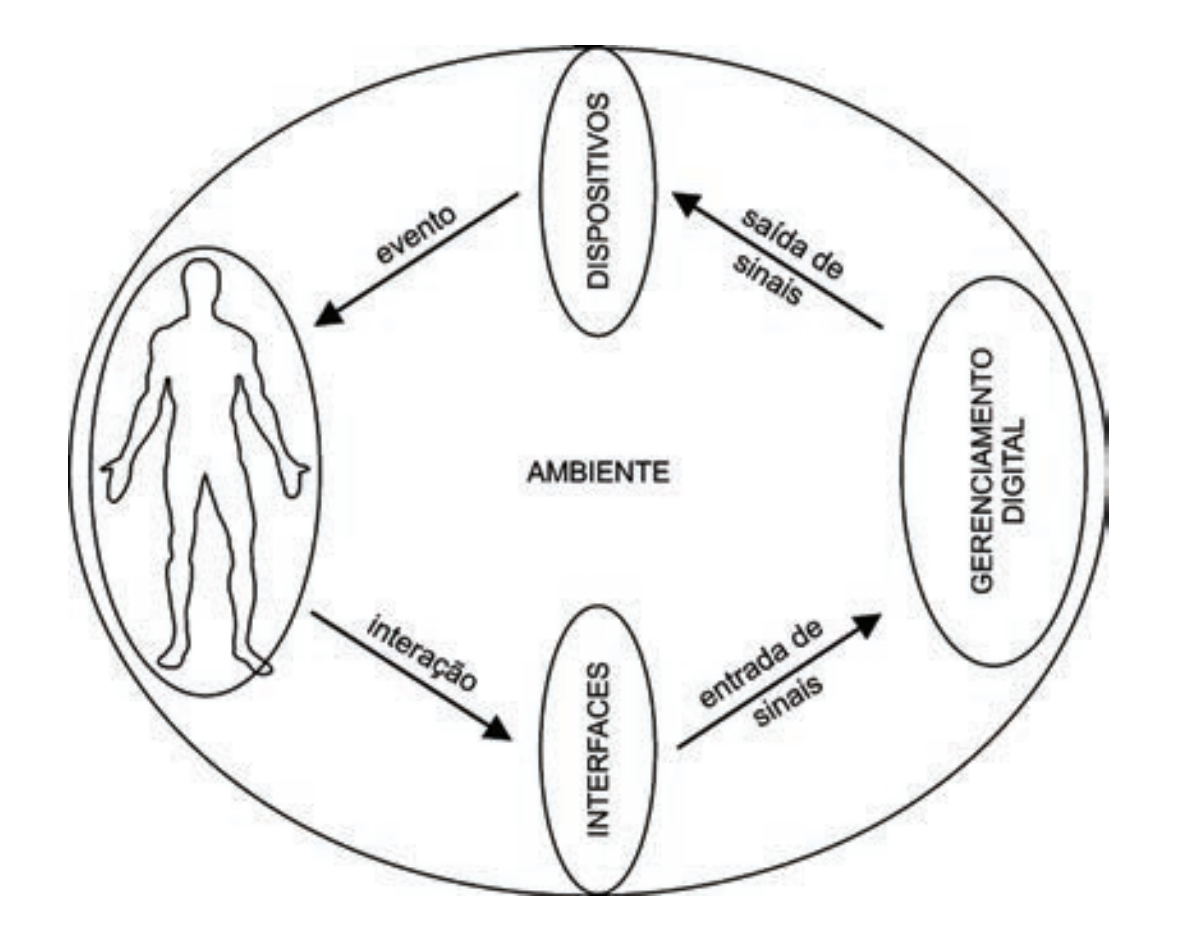
\includegraphics[width=0.8\textwidth]{./04-figuras/instalacoes_interativas}
    \label{fig:instalacoes_interativas}
\end{figure}
\vspace*{-0,9cm}
{\raggedright \fonte{\citeonline[p. 62]{sogabe2011}}}\\


O espaço sempre deve ser considerado para que a obra seja, de fato, uma instalação. De acordo com \citeonline[p. 6]{bochio}, no contexto das instalações interativas, o espaço se torna sensível e os movimentos mais sutis do público são capturados, provocando o diálogo com a imagem. A partir da análise realizada por \citeonline[p. 64]{sogabe2011} podemos afirmar que um evento é tudo que acontece dentro deste espaço. São as respostas fornecidas pelo sistema computacional que se materializam por meio dos dispositivos. Para \citeonline{domingues1998} os dispositivos compõem a cenografia, a ambientação, mas acima de tudo acrescentam elementos internos à própria concepção da obra. \citeonline[p. 62]{sogabe2011} afirma que a simples presença do público no espaço, através do andar, ou de alguma ação física, pode gerar alterações no ambiente. Essas alterações (ou interações) são controladas por algum sistema computacional, ou como denomina o autor, através de gerenciamento digital, que recebe as informações (entrada de sinais), processa através de um programa e devolve para o ambiente no formato de informações atualizadas (saída de sinais), provocando um novo ciclo.

Para \citeonline[p. 64]{sogabe2011} a instalação interativa entende o público como essencial para o acontecimento da obra. O interator se torna um elemento físico presente na instalação e que o artista tem de considerar. Público e interatividade estão intimamente conectados tendo em vista que a interação se manifesta em alguma ação proposta pelo interator. \citeonline[p. 6]{bochio} explica, ainda, que

\begin{citacao}
Em seus deslocamentos pelo espaço, o público constrói uma trama de relações com a obra por aproximação, afastamento, retornos, paradas, transformando o que é percebido por ele. Em instalações interativas, além disso, o público tem a possibilidade de agir e interagir com a situação proposta promovendo modificações nas próprias imagens e sons:  há transformações de ordem física e não mais apenas perceptiva – o que caracteriza o termo interativo nas instalações.  \cite[p. 6]{bochio}  
\end{citacao}

De acordo com \citeonline[p. 199]{witt}, para que qualquer tipo de interatividade aconteça, é necesária a existência de uma interface, uma tecnologia que propicie a comunicação entre o sistema e o interator. \citeonline[p. 37]{levy} define interface como sendo "todos os aparatos materiais que permitem a interação entre o universo da informação digital e o mundo ordinário", enquanto \citeonline[p. 66]{sogabe2011} afirma que "a interface é o aparato físico que capta as ações do público na instalação, a parte sensível do sistema tecnológico". \citeonline[p. 66]{sogabe2011} relata também que a interface não é apenas um aparato tecnológico, mas está diretamente relacionada à produção da poética da instalação.  \citeonline[p. 199]{witt} destacam que estas interfaces devem sempre evoluir, num sentido em que se tornem cada vez mais próximas ao nosso corpo, tenham um funcionamento simples de aprender, e que, acima de tudo, sejam capazes de atender às necessidades da obra. Para \citeonline{rabello} a interface permite, através de um canal de mão dupla entre homem e máquina, que a ação do homem, por mais sutil e imperceptível que pareça, seja reconhecida, processada pela máquina e devolvida para o interator. Portanto, as interfaces se tornam um tipo de condutor, estabelecendo a interatividade e convertendo os espectadores em atores dos sistemas. \citeonline[p. 2570]{rabello2011} afirma que é por meio da interface que a troca de informação e a interação se efetiva, conectando o homem à máquina e engendrando uma atividade intensa, na qual dois mundos até então distintos são intimados a se entrecruzar. A interface provoca uma experiência interativa entre agentes, estabelecendo um novo tipo de relação entre o real e o artificial. Parafraseando \citeonline[p. 140]{arantes} podemos dizer que "é a partir da interface com o interator que a obra pode se manifestar". 


\subsection{O CORPO DO OBSERVADOR NAS INSTALAÇÕES INTERATIVAS}
	
Numa época onde se solicita uma atuação corporal do observador dentro da obra de arte para que esta se atualize ou materialize \citeonline[p. 1582]{sogabe} destaca que a condição do corpo do espectador adquire grande importância, pois, numa visão de um todo sistêmico, este se torna elemento constitutivo da obra. De acordo com \citeonline[p. 2568]{vares} "quando conectado, esse corpo possuirá também alterações em sua espacialidade e fisicalidade, pois através das conexões – onde ocorre o encontro entre o orgânico e o inorgânico – seu corpo será aumentado, ampliado". Chega-se, então, em um momento de diálogo tamanho entre arte, telecomunicações e tecnologia que o público, não mais apenas espectador, passa à posição de interator, explicam \citeonline[p. 528]{souza}. 

\citeonline[p. 1585]{sogabe} entende que o diálogo corporal do espectador com a obra sempre existe. Segundo ele, isso ocorre mesmo nas obras de arte mais tradicionais à medida em que o próprio tamanho e a estrutura da obra provocam a aproximação, o afastamento, o andar de um lado ao outro ou o movimentar da cabeça do observador. Diz ainda que

\begin{citacao}
Nas obras mais tradicionais, até antes do modernismo, a postura do observador em geral é sempre de um corpo fixo, quase imóvel, cujos movimentos restringem-se basicamente ao olhar, que percorre a imagem, de acordo com os centros de atenção e composição dos elementos visuais existentes. \cite[p. 1585]{sogabe} 
\end{citacao}

Segundo \citeonline{rabello} a inserção do corpo no espaço artístico foi inicialmente proposta pela arte da participação nos anos 1970 e 80. Nesta época já se articulava uma experiência sensorial por meio da ativação dos sentidos em ambientes cinéticos fosse pela utilização de óculos, pela ação de pisar, deitar ou apertar botões. \citeonline[p. 534]{soares} diz que ao se analisar o comportamento corporal do público diante da obra (considerando a mente como parte do corpo), percebe-se que os artistas intencionalmente vem solicitando uma real aproximação do observador em relação à mesma, até que ela passe a existir na condição de que o fruidor não só esteja presente, como faça parte da obra e, ainda, colabore com a sua realização. Nas palavras de \citeonline[p. 1140]{semeler2015} "o espectador é recrutado por meio da interatividade para que exerça um papel ativo na construção da obra".

Ainda de acordo \citeonline{rabello} a correlação entre o processo interativo e a experiência estética tornou-se mais evidente com o advento das tecnologias digitais à medida que estas solicitam cada vez mais a ação, a movimentação, a vivência e a conexão do homem com o ambiente virtual, promovendo situações distintas dentro de uma dimensão estética. Para \citeonline[p. 37]{couchot} é possível notar que os dispositivos interativos imaginados pelos artistas tendem a solicitar a participação do corpo inteiro. Neste contexto, \citeonline[p. 1587]{sogabe} acrescenta que o corpo da obra já não existe independente do corpo do observador e que a tecnologia digital transforma os ambientes das instalações em ambientes onde o espaço projeta-se para dentro de imagens inteligentes, que se atualizam de acordo com cada participante, o qual denomina interator ou interagente.

\citeonline[p. 2563]{vares} afirma que na interatividade o corpo dos usuários é colocado em contato direto com as tecnologias, fazendo trocas com estas através da emissão e recepção de mensagens, desenvolvendo o processo da obra. Nas palavras de \citeonline[p. 198]{witt}, "a interatividade também proporciona uma fricção: a do corpo do usuário, orgânico, com um sistema tecnológico, artificial". Para \citeonline[p. 2563]{vares}, neste contexto, a realização da obra não pode ser atribuída apenas ao artista, pois o público irá decidir se empresta ou não o seu corpo ao trabalho. Ela acrescenta que existe uma mudança de paradigma da própria experiência corporal tendo em vista que esses experimentos acontecem publicamente, onde qualquer ação executada pelo interator pode ser vista por outras pessoas presentes no espaço, que podem vir a julgá-lo. Esse fato, pode interferir no próprio desenrolar da obra, fazendo com que o usuário se dedique mais ou menos a participar efetivamente da mesma. \citeonline[p. 199]{witt} concluem que durante o processo das obras, o corpo do espectador e o sistema tecnológico, são convidados a trabalhar em conjunto para que a proposta artística tenha sucesso. "Afinal, é ao corpo que pertencem nossas sensações e percepções, que são justamente os campos afetados por instalações interativas"  \cite[p. 199]{witt}.
